\section{Elemente Der Prädikatenlogik}
Die Aussagenlogik ist eine heile Welt. Aber sie ist zu schwach für die Formulierung und Formalisierung der meisten Mathematischen Tatsachen.\\
\begin{bsp}
	Alle Menschen sind sterblich. \\
	Sokrates ist ein Mensch. \\
	$\drsh$ ? \\
	\begin{itemize}
		\item $\forall x ~ ( \text{Mensch}( x ) \rightarrow \text{Sterblich}( x )$
		\begin{itemize}
			\item Quantisierung über ein Universum.
			\item Prädikate, Eigenschaft $\rightarrow \{ 0 , 1 \}$
			\item Aussagenlogik ( AL ) ist Teil der Prädikatenlogik ( PL ) .
		\end{itemize}
		\item Mensch$($ SOKRATES $)$
			\begin{itemize}
				\item Konstanten
			\end{itemize}
	\end{itemize}
	Mensch$($ SOKRATES $) \rightarrow$ Sterblich$($ SOKRATES $)$
\end{bsp}
\begin{bsp}
	Was ''sagen'' folgende Formeln?\\
	\begin{itemize}
		\item $\forall x \forall \epsilon \exists \delta \forall y~( d( x, y )  < \delta \rightarrow d( f( x ) , f( y ) ) < \epsilon )$
		\begin{itemize}
			\item Quantoren: Universum z.B. $\mathbb{R}^{>0}$
			\item Interpretation von: \\
			\begin{tabular}{ l l }
				''$<$''		& : $<$			\\
				''$d( x , y )$''	& : $\abs{x-y}$		\\
				''$f( x )$''		& : $f( x ) = x^2$	
			\end{tabular}
		\end{itemize}
		\item $\forall n \exists p \forall a \forall b~(p > n \wedge ( p = a \cdot b \rightarrow a = 1 \oplus b = 1 ) )$
		\begin{itemize}
			\item ''Es gibt unendlich viele Primzahlen.''
			\item Struktur: \\
			\begin{tabular}{ l l }
				Universum	& : $\mathbb{N}$		\\
				''$>$''	& : $>$				\\
				''$\cdot$''	& : $\cdot$			\\
				''$1$''	& : $1 \in \mathbb{N}$	
			\end{tabular}
		\end{itemize}
		\item $\exists n \exists a \exists b \exists c~( n \geq 3 \wedge a^n + b^n = c^n )$
		\begin{itemize}
			\item Struktur:
			\begin{itemize}
				\item Universum: $\mathbb{N}$
				\item $\geq , 3 , ^ , +$ wie üblich
			\end{itemize}
			\item \textbf{grosser fermatscher Satz\index{grosser fermatscher Satz}}
			\item falsch
			\item In der PL ist schon das Auswertensproblem schwierig.
		\end{itemize}
	\end{itemize}
\end{bsp}
\begin{bsp*}
	\begin{gather*}
		\forall x~( x \geq 4 \wedge \exists y~( x = 2 \cdot y ) \\
		\quad \rightarrow \exists p \exists q~( x = p + q \wedge \Prim( p ) \wedge \Prim( q ) ) ) \\
		\Prim( r ) \coloneqq ( r = a \cdot b \rightarrow a = 1 \oplus b = 1 )
	\end{gather*}
	\begin{itemize}
		\item Struktur:
		\begin{itemize}
			\item Universum: $\mathbb{N}$
			\item ''übliche'' Interpretationen:
			\begin{itemize}
				\item Konstanten: $1 , 2 , 4$
				\item Funktionen: $+ , \cdot$
				\item Prädikate: $\geq , ( = )$
			\end{itemize}
		\end{itemize}
		\item Allen geraden Zahlen $\geq 4$ können als Summe zweier Primzahlen geschrieben werden. ( \textbf{Goldbach-Vermutung\index{Goldbach-Vermutung}} )
		\item Niemand weiss, ob diese Struktur ein Modell ist für die Formel.
	\end{itemize}
\end{bsp*}
\begin{bem}
	\begin{tabular}{ l l }
		Struktur $\models$ Formel		& ( ist ein Modell )		\\
		$F \models G$				& (semantische Folgerung)	\\
		$F \equiv G$				& (semantische Äquivalnez)	\\
		Tautologie (=gültige Formel):	& jede Struktur ist Modell	\\
		Unerfüllbare Formel:			& keine Struktur ist Modell	
	\end{tabular}
\end{bem}
\begin{bsp*}{Äquivalenzen und gültigen Formeln}
	\begin{itemize}
		\item $\forall x~( P( x ) ) \rightarrow P( c ) \qquad \forall x~( P( x ) ) \models P( c )$
		\item $P( c ) \rightarrow \exists x~( P( x ) ) \qquad ( c ) \models \exists x~( P( x ) )$
		\item $\neg \forall x~( P( x ) ) \equiv \exists x~( P( x ) )$
		\item $\neg \exists x~( P( x ) ) \equiv \forall x~( P( x ) )$
		\item $\forall x~( P( x ) \wedge Q( x ) ) \equiv \forall x~( P( x ) ) \wedge \forall x~( Q( x ) ) \equiv \forall x~( P( x ) ) \wedge \forall y~( Q( y ) )$
		\item $\exists x~( P( x ) \vee Q( x ) ) \equiv \exists x~( P( x ) ) \vee \exists x~( Q( x ) ) \equiv \exists x~( P( x ) ) \vee \exists y~( Q( y ) )$
		\item $\forall x~( P( x ) \vee Q( x ) ) \Leftarrow \forall x~( P( x ) ) \vee \forall y~( Q( y ) )$  \quad \textbf{ABER NICHT UMGEKEHRT} (mögliche Interpretation: ''Alle Zahlen sind gerade oder ungerade.'' )
		\item $\exists x~( P( x ) \wedge Q( x ) ) \Rightarrow \exists x~( P( x ) ) \wedge \exists y~( Q( y ) )$  \quad \textbf{ABER NICHT UMGEKEHRT} (mögliche Interpretation: ''retation: Es gibt gerade und es gibt ungerade Zahlen.'' )
		\item $\forall x \forall y P( x , y ) \equiv \forall y \forall x P( x , y )$
		\item $\exists x \exists y P( x , y ) \equiv \exists y \exists x P( x , y )$
		\item $\forall x \exists y P( x , y ) \Leftarrow \exists y \forall x P( x , y )$ \quad \textbf{ABER NICHT UMGEKEHRT}
	\end{itemize}
\end{bsp*}

\subsection{Ist das Erfüllbarkeitsprobelm der PL algorithmisch entscheidbar?}
\begin{itemize}
	\item AL \\
		\[
			F \text{ erfüllbar } \rightarrow \begin{array}{l}
				\text{Algorithumus}		\\
				\text{Wahrheitstabelle}	\\
				\text{Resolution}			
			\end{array} \begin{array}{l}
				\rightarrow \text{ ''ja''}		\\
				\rightarrow \text{ ''nein''}	
			\end{array} \qquad \qquad \textbf{entscheidbar}
		\]
	\item PL \\
	\begin{gather*}
		F \text{ erfüllbar } \rightarrow \text{ jede mögliche Struktur einsetzen} \begin{array}{l}
			\rightarrow \text{\Interval} \\
			\rightarrow \text{\Interval}
		\end{array} \\
		F \text{ erfüllbar } \rightarrow \text{ ''Resolution'', Unifikation} \begin{array}{l}
			\rightarrow \text{\Interval} \\
			\rightarrow \text{''nein''}
		\end{array} \textbf{semi-entscheidbar}
	\end{gather*}
\end{itemize}
Ist die PL entscheidbar? \\
\textbf{NEIN}\\
Sie wäre es, wenn es möglich wäre, zu ntscheiden, ob ein gegebener Algorithmus auf einem gegebenen Input abhält.\\
Halteproblem:
\begin{itemize}
	\item Annahme: Es geht.
	\item 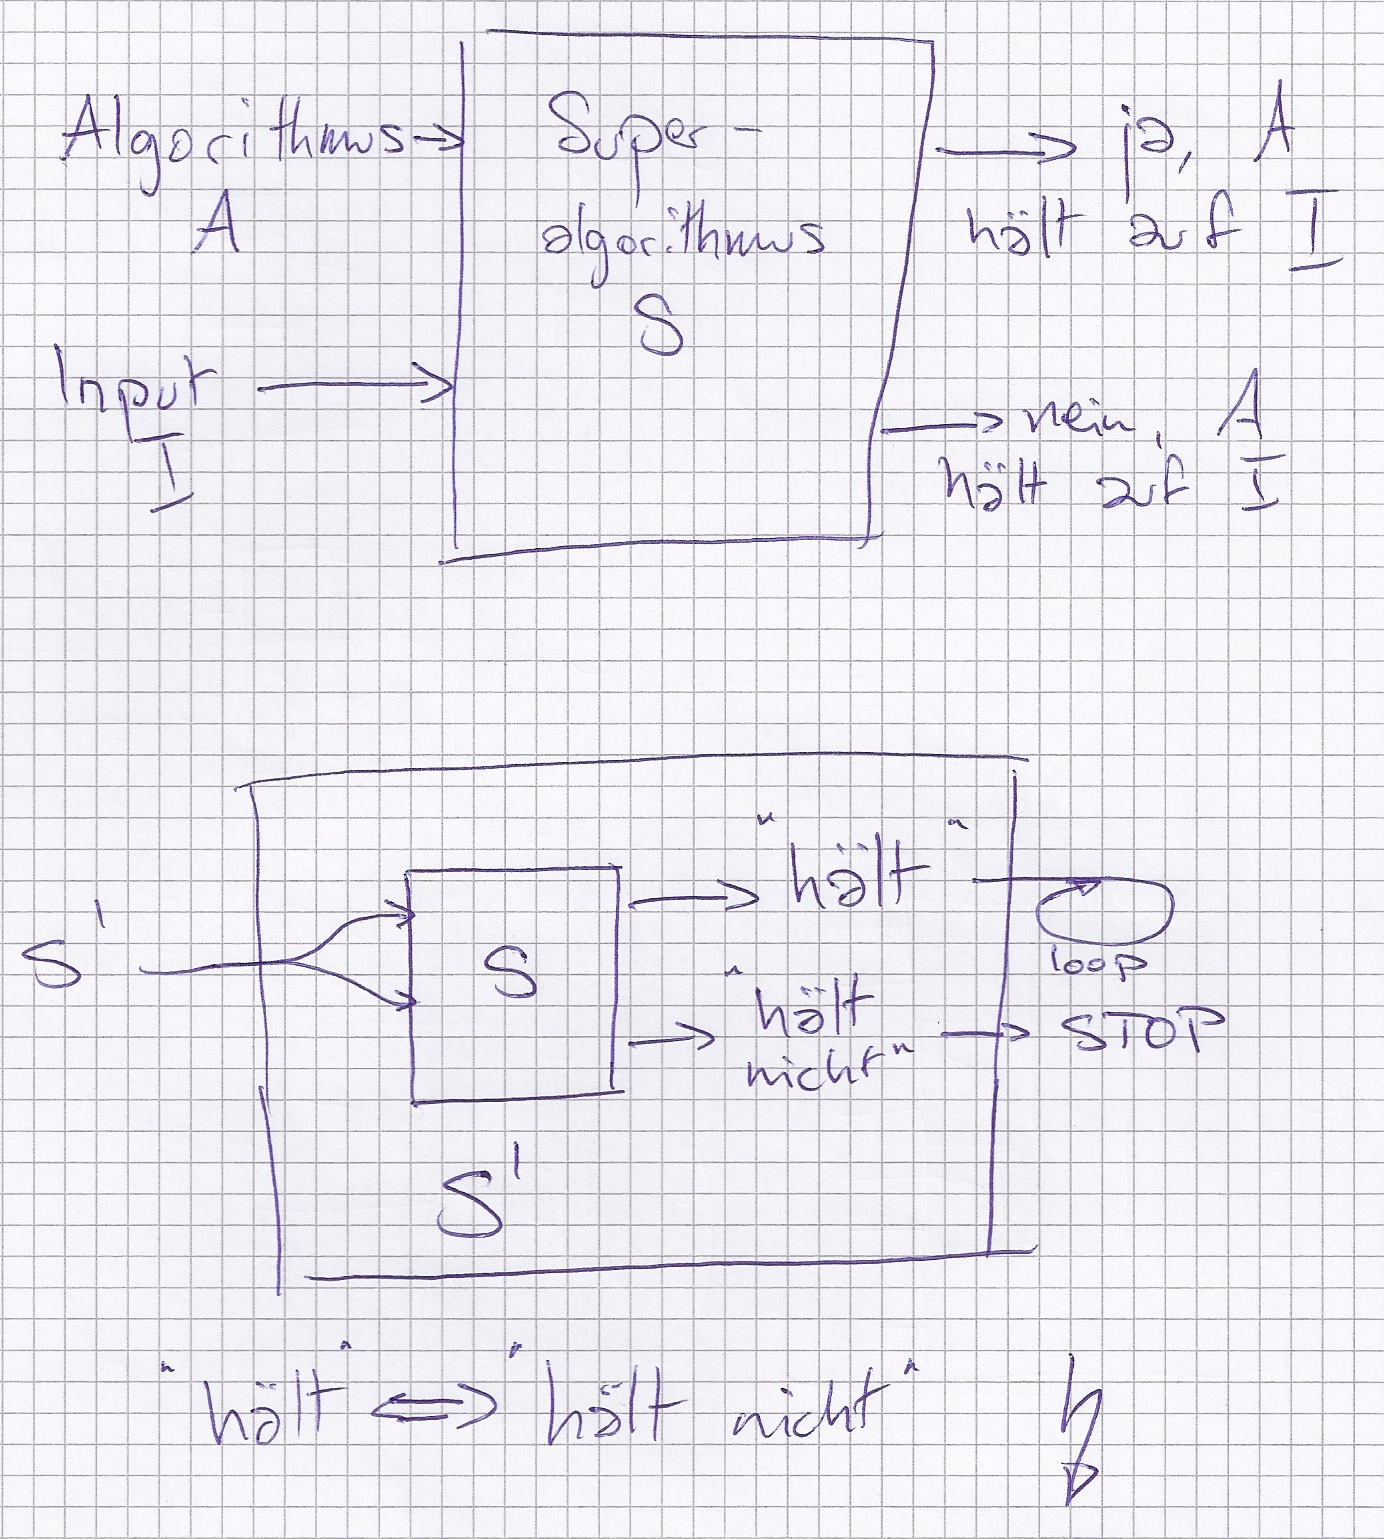
\includegraphics[width=\textwidth]{Bild14}
	\item Das Halteproblem ist nicht entscheidbar $\implies$ die PL ist nicht entscheidbar.
\end{itemize}

\subsection{Selbstbezüglichkeit als Quelle von Paradoxa, Einsichten, Katostrophen}
\begin{itemize}
	\item (Hofstadter)
	\item Epinemides (aus Kreta): ''Alle Kreter sind Lügner.''
	\begin{itemize}
		\item ''Ich bin falsch.''
	\end{itemize}
	\item Wie viele Buchstaben hat die Antwort auf diese Frage?
	\begin{itemize}
		\item Vier
	\end{itemize}
	\item ''Die kleinste Zahl, die sich nicht durch einen deutschen Satz mit höchstens zwanzig Wörtern beschreiben lässt.''
	\begin{itemize}
		\item 16
	\end{itemize}
	\item Gödel:
	\begin{itemize}
		\item Hilberts Traum: Formales System, in dem alles richtige beweisbar ist. $\eqqcolon \Delta$
		\item Formeln $F$ und Beweise $B$ sind Strings / natürliche Zahlen.
		\item Prädikat $Abl( B, F )$ \qquad ''B beweist F.''
		\item $F_i( x ) , i = 1 , 2 , \dotsc$ \qquad Alle Formeln mit Variable $x$.
		\item $\neg \exists B~( Abl( B , F_x( x ) ) = F_{i_0}( x )$
		\item $\neg \exists B~( Abl( B , F_{i_0}( i_0 ) ) = F_{i_0}( i_0 )$
	\end{itemize}
\end{itemize}
